\subsection{tx\_packet}
The {\bf tx\_packet\_str} is a abstraction of a TX packet structure. 
Most of the functions are used to set the FCF field in TX packet. FCF has two bytes in length
and each bits represent different information. Figure~\ref{fig:FCF} gives a brief view of FCF
field. A tx packet contains header and payloads. {\bf tx\_packet\_str } stores most of the header 
information except the {\bf source address}, {\bf source address mode} and {\bf source PAN ID}.
These information can be retrieved by a pointer to a radio ({\bf rp}) structure which owns this 
tx packet. Also, {\bf data\_ptr} is the pointer to the payload.
\begin{figure}[h]
	\centering
	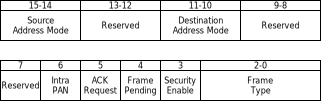
\includegraphics[width=0.6\columnwidth]{FCF}
	\caption{Detail information of FCF field}
	\label{fig:FCF}
\end{figure}

\begin{lstlisting}[language=c, caption=TX Packet Structure]
	struct tx_packet_str{
		uint8_t frame_type;
		uint8_t security_en;
		uint8_t frame_pending;
		uint8_t ack_req;
		uint8_t intra_pan;
		uint8_t dest_addr_mode;
		uint8_t dsn;
		uint16_t dest_pan_ID;
		uint32_t dest_addr_LSB, dest_addr_MSB;
		uint8_t pkt_overhead;
	
		uint8_t data_length;
		uint32_t* data_ptr;
		struct radio* rp;
	};
\end{lstlisting}

\begin{enumerate}
	\item inline uint8\_t set\_dest\_addr\_mode(struct tx\_packet\_str* tp, uint8\_t dam);
	\item inline void set\_pan\_id\_comp(struct tx\_packet\_str* tp, uint8\_t ip);
	\item inline void set\_ack(struct tx\_packet\_str* tp, uint8\_t ar);
	\item inline void set\_frame\_pending(struct tx\_packet\_str* tp, uint8\_t fp);
	\item inline void set\_security(struct tx\_packet\_str* tp, uint8\_t se);
	\item inline void set\_frame\_type(struct tx\_packet\_str* tp, uint8\_t ft);
	\item inline void set\_DSN(struct tx\_packet\_str* tp, uint8\_t DSN);
	\item inline void set\_dest\_pan(struct tx\_packet\_str* tp, uint16\_t dp);
	\item inline void set\_dest\_addr(struct tx\_packet\_str* tp, uint32\_t da1, uint32\_t da0);
	\item void calculate\_FCF(struct tx\_packet\_str* tp, uint32\_t* tx\_pkt\_ptr);
	\item uint8\_t calculate\_address(struct tx\_packet\_str* tp, uint32\_t* tx\_pkt\_ptr);
	\item uint8\_t data\_trans (struct tx\_packet\_str* tp);
\end{enumerate}

\subsubsection{inline uint8\_t set\_dest\_addr\_mode(struct tx\_packet\_str* tp, uint8\_t dam)}
\hangindent=\parindent
\hangafter=0
Input argument: tx\_packet\_str pointer, destination address mode (dam).\\
Return value: Success/Fail. 0: Fail, 1: Success.\\
\begin{table}[h]
\centering
	\begin{tabular}{|c|c|}
	\hline
	{\bf Source/Destination Address Mode} & {\bf Address Field Length}\\ \hline
	0 & No PAN/Address present\\ \hline
	2 & 2 Bytes\\ \hline
	3 & 8 Bytes\\ \hline
	\end{tabular}
	\caption{List of destination address mode}
	\label{tab:address_mode}
\end{table}

\subsubsection{inline void set\_pan\_id\_comp(struct tx\_packet\_str* tp, uint8\_t ip)}
\hangindent=\parindent
\hangafter=0
Input argument: tx\_packet\_str pointer, Intra PAN (ip)\\
Return value: None\\
"The PAN ID Compression subfield is 1 bit in lengthand specifies whether the MAC frame is to 
be sent containing only one of the PAN identifier fields whenboth source and destination 
addresses are present"~\cite{802.15.4.standard}
The available options are following:
\begin{table*}[h]
\centering
\begin{threeparttable}
	\begin{tabular}{|c|c|c|c|c|}
	\hline
	{\bf Intra PAN} & {\bf Dest. PAN} & {\bf Dest. Addr.} & {\bf Source PAN} & {\bf Source Addr.}\\ \hline
	1 & Present			& Present			& None~\tnote{a}	& Present\\ \hline
	0 & Present			& Present			& Present			& Present\\ \hline
	0 & Present			& Present			& None~\tnote{b}	& None~\tnote{b}\\ \hline
	0 & None~\tnote{b}	& None~\tnote{b}	& Present			& Present\\ \hline
	0 & None~\tnote{b}	& None~\tnote{b}	& None~\tnote{b}	& None~\tnote{b}\\ \hline
	\end{tabular}
	\begin{tablenotes}
		\item [a] Source PAN ID. equals to Destination PAN ID.
		\item [b] Refer table~\ref{tab:address_mode} for detail information.
	\end{tablenotes}
\end{threeparttable}
	\caption{PAN ID compression and source/destination address mode}
\end{table*}

\subsubsection{inline void set\_ack(struct tx\_packet\_str* tp, uint8\_t ar)}
\hangindent=\parindent
\hangafter=0
Input argument: tx\_packet\_str pointer, ACK request (ar)\\
Return value: None\\
\begin{table}[h]
\centering
	\begin{tabular}{|c|c|}
	\hline
	{\bf ACK request (ar)} & {\bf Effect}\\ \hline
	0 & No ACK\\ \hline
	1 & Request ACK\\ \hline
	\end{tabular}
	\caption{ACK Request}
\end{table}
Note that the ACK request bit should not be set in broadcast~\footnote{
Destination address \= 0xffff or 0xffffffffffffffff} packet.


\subsubsection{inline void set\_frame\_pending(struct tx\_packet\_str* tp, uint8\_t fp)}
\hangindent=\parindent
\hangafter=0
Input argument: tx\_packet\_str pointer, frame pending(fp)\\
Return value: None\\
\begin{table}[h]
\centering
	\begin{tabular}{|c|c|}
	\hline
	{\bf frame pending (fp)} & {\bf Effect}\\ \hline
	0 & No frame pending\\ \hline
	1 & Frame pending\\ \hline
	\end{tabular}
	\caption{Frame Pending}
\end{table}

\subsubsection{inline void set\_security(struct tx\_packet\_str* tp, uint8\_t se)}
\hangindent=\parindent
\hangafter=0
Input argument: tx\_packet\_str pointer, Security Enable (se)\\
Return value: None\\
\begin{table}[h]
\centering
	\begin{tabular}{|c|c|}
	\hline
	{\bf Security Enable (se)} & {\bf Effect}\\ \hline
	0 & Security Enable\\ \hline
	1 & Security Disable\\ \hline
	\end{tabular}
	\caption{Security enable}
\end{table}

\subsubsection{inline void set\_frame\_type(struct tx\_packet\_str* tp, uint8\_t ft)}
\hangindent=\parindent
\hangafter=0
Input argument: tx\_packet\_str pointer, Frame Type (ft)\\
Return value: None\\
\begin{table}[h]
\centering
	\begin{tabular}{|c|c|}
	\hline
	{\bf Frame Type (ft)} & {\bf Effect}\\ \hline
	0 & Beacon\\ \hline
	1 & Data\\ \hline
	2 & Acknowledgment\\ \hline
	3 & Mac Command\\ \hline
	\end{tabular}
	\caption{Frame type}
\end{table}

\subsubsection{inline void set\_DSN(struct tx\_packet\_str* tp, uint8\_t DSN)}
\hangindent=\parindent
\hangafter=0
Input argument: tx\_packet\_str pointer, Data Sequence Number (DSN)\\
Return value: None\\
This function sets the DSN field in a TX packet.


\subsubsection{inline void set\_dest\_pan(struct tx\_packet\_str* tp, uint16\_t dp)}
\hangindent=\parindent
\hangafter=0
Input argument: tx\_packet\_str pointer, Destination PAN ID (dp)\\
Return value: None\\
This function sets the destination PAN ID in a TX packet.


\subsubsection{inline void set\_dest\_addr(struct tx\_packet\_str* tp, uint32\_t da1, uint32\_t da0)}
\hangindent=\parindent
\hangafter=0
Input argument: tx\_packet\_str pointer, Destination Address (da1, da0)\\
Return value: None\\
This function sets the destination address in a TX packet. Destination address could be as
long as 8 bytes (destination address mode = 3). If 8 bytes mode is selected, destination
address = {da1 (higher 32-bits), da0 (lower 32-bits)}. Similarly, destination address = 
(da0 \& 0xffff) if 2 bytes mode is selected.

\subsubsection{void calculate\_FCF(struct tx\_packet\_str* tp, uint32\_t* tx\_pkt\_ptr)}
\hangindent=\parindent
\hangafter=0
Input argument: tx\_packet\_str pointer, TX packet header pointer\\ 
Return value: None\\
This function aggregates all the settings to 2 bytes FCF field.

\subsubsection{uint8\_t calculate\_address(struct tx\_packet\_str* tp, uint32\_t* tx\_pkt\_ptr)}
\hangindent=\parindent
\hangafter=0
Input argument: tx\_packet\_str pointer, TX packet header pointer\\ 
Return value: 
This function calculates address format in a TX packet by source/destination
address mode and Intra PAN ID bit.

\subsubsection{uint8\_t data\_trans (struct tx\_packet\_str* tp)}
\hangindent=\parindent
\hangafter=0
Input argument: tx\_packet\_str pointer\\ 
Return value: Success/Fail. 0: Fail, 1: Success.\\
This function initiates a PDMA transfer which load the packet into TX fifo.
